\chapter{万花尺\label{ch02}}
\section{参数方程}
\subsection{万花尺方程}
\autoref{fig2-3} 展示了类似万花尺运动的数学模型。

\begin{figure}
    \centering
    \begin{subfigure}[b]{.45\textwidth}
        \centering
        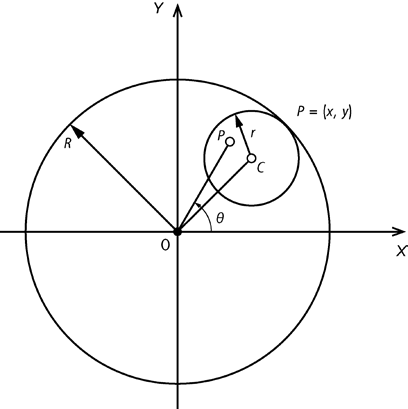
\includegraphics[width=\textwidth]{../img/fig2-3.png}
        \caption{万花尺数学模型}
        \label{fig2-3}
    \end{subfigure}
    \hfill
    \begin{subfigure}[b]{.45\textwidth}
        \centering
        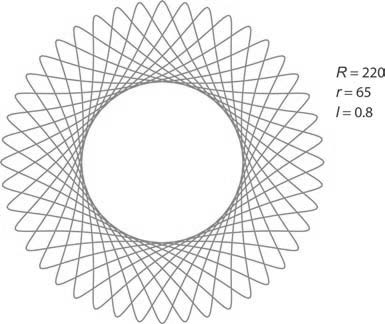
\includegraphics[width=\textwidth]{../img/fig2-4.png}
        \caption{示例曲线,$R=220,~r=65,~l=0.8$}
        \label{fig2-4}
    \end{subfigure}
    \caption{万花尺和某个示例}
\end{figure}

在 \autoref{fig2-3} 中,$C$ 是较小的圆的圆心,$P$ 是笔尖。较大的圆半径为 $R$,较小的圆半径为 $r$。半径之比表示如下:
$$k=\frac{r}{R}$$

将线段 $PC$ 与小圆半径 $r$ 之比作为变量 $l$($l = PC / r$),它决定了笔尖离小圆圆心有多远。然后,组合这些变量来表示 $P$ 的运动,得到如下的参数方程:
\begin{equation}
    \begin{aligned}
        x & =R\left((1-k)\cos(\theta)+lk\cos\left(\frac{1-k}{k}\theta\right)\right) \\
        y & =R\left((1-k)\sin(\theta)+lk\sin\left(\frac{1-k}{k}\theta\right)\right) \\
    \end{aligned}
\end{equation}

将曲线绘制为一系列点之间的线段。如果这些点足够接近,图看起来就像平滑的曲线。

要确定何时停止绘图,就要利用万花尺的周期性(即万花尺图案多久开始重复),研究内外圆的半径之比:
$$\frac{r}{R}$$

分子分母除以它们的最大公约数(GCD),化简该分数,分子就告诉我们需要多少圈才能完成曲线。例如,在 \autoref{fig2-4} 中,$(r, R)$ 的 GCD 是 5。
$$\frac{r}{R}=\frac{65}{220}$$
下面是该分数化简后的形式:
$$\frac{(65/5)}{(220/5)}=\frac{13}{44}$$

这告诉我们,13 圈后,曲线将开始重复。44 告诉我们小圆围绕其中心旋转的圈数,它提示了曲线的形状。在 \autoref{fig2-4} 中数一下,会看到图形中花瓣或叶的数目恰好是 44!

一旦用简化形式表示了半径比 $r/R$,画出螺线的参数 $\theta$ 范围就是 $[0, 2\pi r]$。这告诉我们何时停止绘制特定的螺线。不知道该角度的结束范围,就会循环不止,不必要地重复该曲线。

